%-------------------------------------------------------------------------------
% seq66_menu
%-------------------------------------------------------------------------------
%
% \file        seq66_menu.tex
% \library     Documents
% \author      Chris Ahlstrom
% \date        2015-08-31
% \update      2019-08-20
% \version     $Revision$
% \license     $XPC_GPL_LICENSE$
%
%     Provides the Menu section of sequencer66-user-manual.tex.
%
%-------------------------------------------------------------------------------

\section{Menu}
\label{sec:seq66_menu}

   The \textsl{Sequencer66} menu
   (\figureref{fig:seq66_main_screen}) is simple, but important.

\subsection{Menu / File}
\label{subsec:seq66_menu_file}

   The \textbf{File} menu is used to save and load MIDI files
   (Standard MIDI Format 0 or 1) and \textsl{Sequencer66} MIDI
   files.
   The \textsl{Sequencer66} menu entry contains the sub-items shown below.
%  \figureref{fig:seq66_menu_file_items}.
   The next few sub-sections discuss
   the sub-items in the \textsl{File} sub-menu.

\begin{figure}[H]
   \centering 
   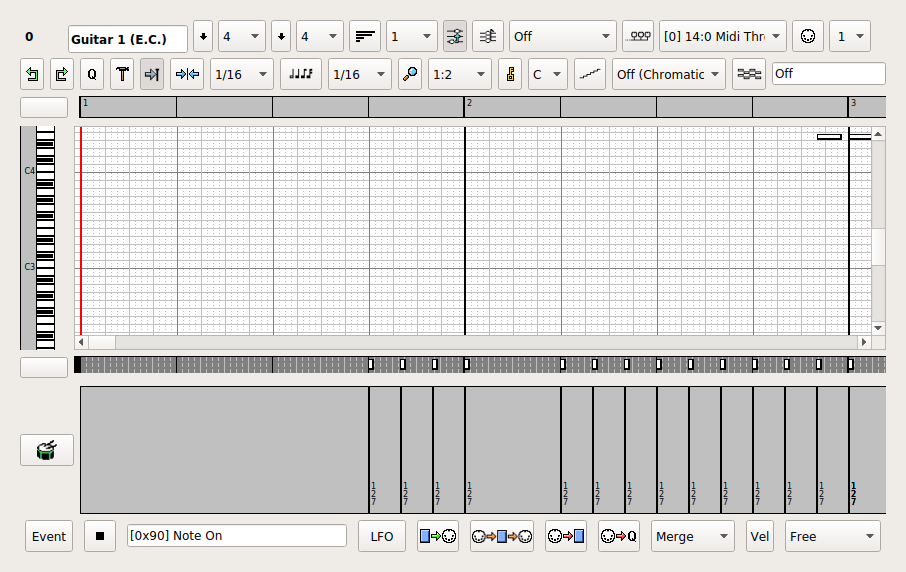
\includegraphics[scale=0.65]{roll.png}
   \caption{Sequencer66 File Menu Items}
   \label{fig:seq66_menu_file_items}
\end{figure}

   \begin{enumber}
      \item \textbf{New}
      \item \textbf{Open}
      \item \textbf{Open Playlist}
      \item \textbf{Recent MIDI files}
      \item \textbf{Save}
      \item \textbf{Save As}
      \item \textbf{Export Song as MIDI}
      \item \textbf{Export MIDI Only}
      \item \textbf{Import MIDI to Current Set}
%     \item \textbf{Options}
      \item \textbf{Exit or Quit}
   \end{enumber}

%  The Qt version of this menu is similar, except that the
%  \textbf{Options...} menu is placed in \textbf{Edit / Preferences}.

\subsection{Menu / File / New}
\label{subsec:menu_file_new}

   The \textbf{New} menu entry clears out the current song or play-list.
   If unsaved changes are pending, the user is prompted to save the changes.
   Prompting for changes is more comprehensive than \textsl{Seq24}.
   However, when in doubt, save!  Keep backups of your tunes!

\subsubsection{Menu / File / Open}
\label{subsubsec:seq66_menu_file_open}

   The \textbf{Open} menu entry opens a song (MIDI file or \textsl{Cakewalk}
   WRK file), replacing the current song.
   It opens up a standard Qt 5 file dialog:

\begin{figure}[H]
   \centering 
%  \includegraphics[scale=0.5]{menu/menu_file_open.png}
   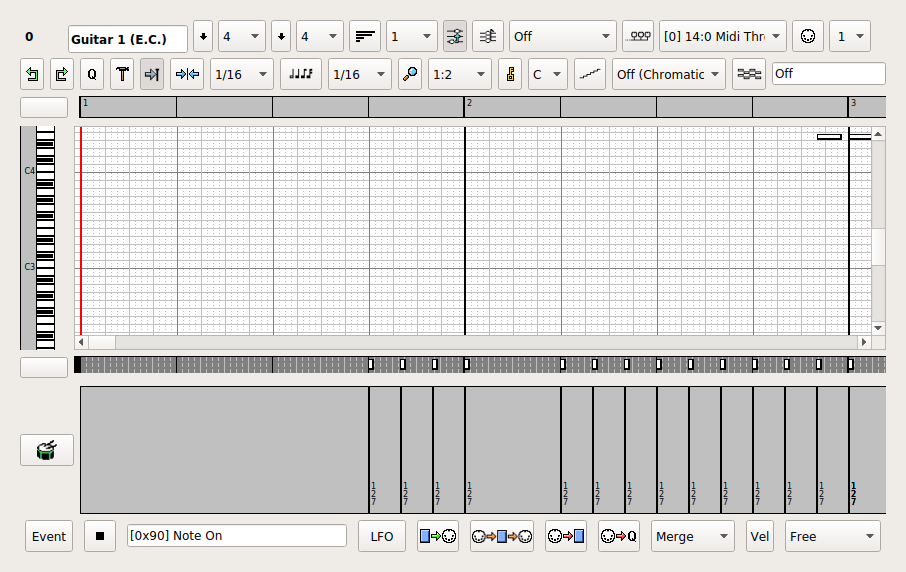
\includegraphics[scale=0.65]{roll.png}
   \caption{File / Open}
   \label{fig:seq66_menu_file_open}
\end{figure}

   This dialog lets one type a file-name, highlighting the first file (if any)
   that matches the characters typed so far.
   \textsl{Sequencer66} can open regular MIDI files and
   Cakewalk WRK files.
   It will read and store some MIDI Meta events 
   (e.g. Tempo and Time Signature).

\subsubsection{Menu / File / Open Playlist}
\label{subsubsec:seq66_menu_file_open}

   The \textbf{Open Playlist...} menu entry opens a \textsl{Sequencer66}
   play-list file.
   This file contains a list of "playlist sections",
   each listing a number of MIDI songs.
   These playlists and songs can be
   selected by the arrow keys or by MIDI control.
   See \sectionref{sec:playlist}.

   Once activated, the current play-list file-name is saved in the
   \texttt{[playlist]} section of the "rc" configuration file when
   \textsl{Sequencer66} exits.
   The file extension is \texttt{.playlist}.
   The Qt user-interface will eventually support editing of the play-list.
   Currently, the user must understand the play-list format, and use a
   text editor to edit the play-list file.

\subsubsection{Menu / File / Recent MIDI files}
\label{subsubsec:seq66_menu_file_recent}

   This menu entry provides a list of the last few MIDI files created or opened;
   play-list selections are \textsl{not} included.
   This list is saved in the \texttt{[recent-files]} section of the
   "rc" configuration file.
   In the menu, only the last part of the file-name is
   shown, but in the "rc" configuration file,
   the full path to the file-name is stored.
   This path is in "UNIX" format, using the forward slash, or solidus,
   as the path separator, even in \textsl{Windows}.
   Only unique entries are included in the recent-files list.
   The limit is 10 recent-file entries.
   This is a feature from \textsl{Kepler34} (\cite{kepler34}).
   Here is an example from an "rc" file:

\begin{verbatim}
   [recent-files]
   # Holds a list of the last few recently-loaded MIDI files.
   3
   /home/chris/git/seq66/data/b4uacuse-gm-patchless.midi
   /home/chris/git/seq66/contrib/midi/colours.midi
   /home/chris/git/seq66/Julian-data/TestBeeps.midi
\end{verbatim}

\subsubsection{Menu / File / Save and Save As}
\label{subsubsec:menu_file_open_save_as}

   The \textbf{Save} menu entry saves the song under its current file-name.
   If there is no current file-name, it opens up a standard file
   dialog to name and save the file.
   The \textbf{Save As} menu entry saves a song under a different name.
   It opens up the following standard file dialog, very similar to the 
   \textbf{File Open} dialog, with an additional \textbf{Name} text-edit field.

\begin{figure}[H]
   \centering 
%  \includegraphics[scale=0.5]{menu/menu_file_save_as.png}
   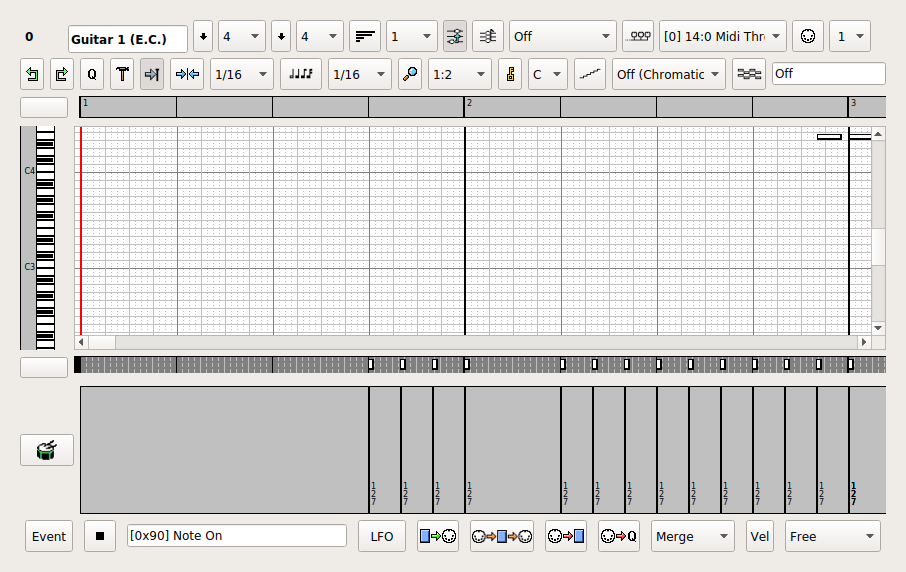
\includegraphics[scale=0.65]{roll.png}
   \caption{File / Save As}
   \label{fig:seq66_menu_file_save_as}
\end{figure}

   To save a new file, or to save the current existing file to a new name,
   enter the name in the name field, without an extension.
   \textsl{Sequencer66} will append a \texttt{.midi} extension to the filename.
   The file will be saved in a format that the Linux \textsl{file} command
   will tag as something like:

   \begin{verbatim}
      myfile.midi: Standard MIDI data (format 1) using 16 tracks at 1/192
   \end{verbatim}

   It looks like a simple MIDI file, and yet, if one re-opens it in
   \textsl{Sequencer66}, one sees that all of the labeling, pattern
   information, and song layout has been preserved in this file.
%  Even the pattern layout (arrangement), as discussed in
%  \sectionref{subsubsec:seq66_song_editor_arrangement_panel_roll},
%  have been saved.
%  (But the L and R marker positions are not saved.)
   This information is saved in a way that MIDI-compliant software
   should be able to use, or ignore without failure.

   The output MIDI file after \textsl{Sequencer66} saves the original MIDI file
   is larger.
   After the last track in the file, a number of
   \index{SeqSpec}
   MIDI-compliant sequencer-specific (SeqSpec) items are saved, to preserve
   the extra information that \textsl{Sequencer66} adds.
   In legacy mode, \textsl{Sequencer66} saves this information
   in the same format as \textsl{Seq24}.
   Otherwise, it saves it in a more MIDI-compatible format.
%  Some of this extra information (mute-groups) will be stripped from the MIDI
%  file.
   Normally, \textsl{Sequencer66} saves this information by marking
   each SeqSpec section as vendor-specific information, and marking this
   section as a regular MIDI track.
   The legacy and new formats of the final "track" are explained in
   \sectionref{subsec:legacy_midi_format}.

   \index{Meta events}
   Meta events are now partially handled by \textsl{Sequencer66}.
   Meta events Set Tempo
%  (\texttt{FF 51 03 tt tt tt}),
   and Time Signature
%  (\texttt{FF 58 04 nn dd cc bb}),
   are now fully supported.
   Other Meta events,
   such as Meta MIDI Channel
%  (\texttt{FF 20 01 cc}),
   and Meta MIDI Port
%  (\texttt{FF 21 01 pp}),
   are now read as events, and are saved back when the file is saved.
   They cannot be edited in \textsl{Sequencer66}, but they are
   not lost.
   Please note that the channel and port meta events are
   considered \textsl{obsolete} in the MIDI standard.

\subsubsection{Menu / File / Import MIDI}
\label{subsubsec:seq66_menu_file_import}

   The \textbf{Import} menu entry imports an SMF 0
   or SMF 1 MIDI file as one or more patterns, one pattern per track,
   into the specified screen-set.
   This functionality is explained in detail in
   \sectionref{subsec:seq66_midi_export_file_import}.

\subsubsection{Menu / File / Export Song as MIDI}
\label{subsubsec:seq66_menu_file_export}

   Thanks to the \textsl{Seq32} project, the ability to export songs to MIDI
   format has been added.  In this export, a complete song performance is
   recoded so that other MIDI sequencers can play the performance properly.
   This functionality is explained in detail in
   \sectionref{subsec:seq66_midi_export_file_export}.

\subsubsection{Menu / File / Export MIDI Only}
\label{subsubsec:seq66_menu_file_export_midi_only}

   Sometimes it might be useful to export only the non-sequencer-specific
   (non-SeqSpec) data from a \textsl{Sequencer66} song, in order to reduce the
   size of the file or to accomodate non-compliant sequencers.
   This functionality is explained in detail in
   \sectionref{subsec:seq66_midi_export_file_export_midi_only}.

\subsubsection{Menu / File / Options}
\label{subsubsec:seq66_menu_file_options}

   In the \textsl{Portmidi / Windows / Qt 5} version of
   \textsl{Sequencer66}, the \textbf{Options} dialog has been moved to 
   \textbf{Edit / Preferences}.
   See \sectionref{subsubsec:qt_portmidi_qt5_edit_prefs}.
   There are still a few configuration items yet to be represented in that
   new user-interface.

   \textbf{Options} provides a number of settings in one
   tabbed dialog, shown in the figures that follow.
   It allows one to set MIDI clocking,
   what incoming MIDI events control the sequencer, what keys are
   mapped to functions, how the mouse works, and some JACK parameters.
   Note that there is a new tab-page for \textbf{Ext Keys}, to support
   more keystroke controls.

\begin{figure}[H]
   \centering 
%  \includegraphics[scale=0.65]{menu/options-tab-0-9-18.png}
   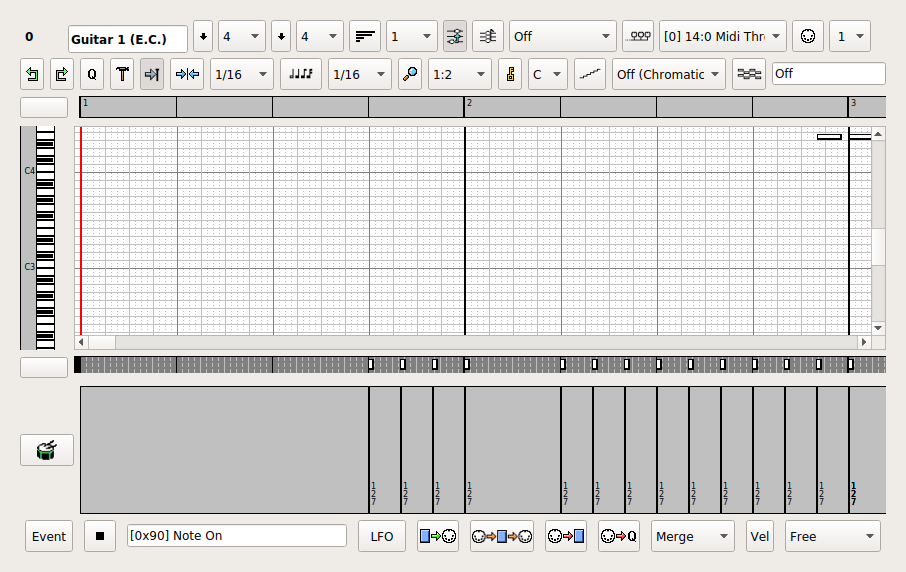
\includegraphics[scale=0.65]{roll.png}
   \caption{Edit / Preference}
   \label{fig:seq66_options_tab_0_9_18}
\end{figure}

\paragraph{Menu / File / Options / MIDI Clock}
\label{paragraph:seq66_menu_file_options_midi_clock}

   The \textbf{MIDI Clock} tab provides a way to set MIDI clock for
   the available MIDI output busses.
   It configures to what busses the MIDI clock and data gets dumped.
   It also shows the devices that can play music.
   The items that appear in this tab depend the setup.

   \begin{itemize}
      \item What MIDI devices are connected to the computer.
         MIDI controllers, USB MIDI cables, applications with virtual
         ports, and other connected devices will add MIDI
         output devices (ports) to the system.
         In \textsl{Windows}, the available devices are shown as well.
%     \item What MIDI software applications are running on the computer.
%        For example, running MIDI software synthesizers such as
%        \textsl{Timidity} and \textsl{Yoshimi} will add extra output devices
%        (playback ports) to a system.
      \item The setting of the "manual-ports" option, which tells
         \textsl{Sequencer66} to set up virtual MIDI ports.
         It is enabled by the
         \texttt{--manual-ports} command-line option or the
         \texttt{[manual-ports]} section of the
         \texttt{sequencer66.rc} configuration file, described in
         \sectionref{subsec:seq66_rc_file_manual_ports}.
      \item The setting of the \textsl{Sequencer66}-specific
         "reveal ALSA ports" option,
         \texttt{--reveal-ports} command-line option or the
         \texttt{[reveal-ports]} section of the
         \texttt{sequencer66.rc} configuration file, described in
         \sectionref{subsec:seq66_rc_file_reveal_ports}.
   \end{itemize}

   For the current discussion, a USB MIDI cable was plugged into the system,
   and the \textsl{Timidity} and \textsl{Yoshimi} (in ALSA mode) software
   synthesizers were running.  \textsl{Sequencer66} was also running,
   without virtual ports enabled, and \texttt{--alsa} turned on.
%  with the option of "manual-ports" (\texttt{-m} or
%  \texttt{--manual-ports}) and ALSA (\texttt{-A} or
%  \texttt{--alsa} turned on.
   Here are the devices shown when running \textsl{aplaymidi}
   from the command-line:

   \begin{verbatim}
      $ aplaymidi -l
       Port    Client name                      Port name
       14:0    Midi Through                     Midi Through Port-0
       24:0    E-MU XMidi1X1 Tab                E-MU XMidi1X1 Tab MIDI 1
      128:0    TiMidity                         TiMidity port 0
      128:1    TiMidity                         TiMidity port 1
      128:2    TiMidity                         TiMidity port 2
      128:3    TiMidity                         TiMidity port 3
      129:0    seq66                            seq66 in
   \end{verbatim}

%     129:16   sequencer66                      sequencer66 in

   Note that \textsl{Yoshimi} does not appear.  Perhaps
   \texttt{aplaymidi} does not subscribe properly to all ALSA notifications.
   A better command might be this one (a different setup than above):

   \begin{verbatim}
      $ aconnect -lio
      client 0: 'System' [type=kernel]
          0 'Timer           '
          1 'Announce        '
         Connecting To: 15:0, 128:0
      client 14: 'Midi Through' [type=kernel]
          0 'Midi Through Port-0'
      client 129: 'yoshimi' [type=user,pid=26335]
          0 'input           '
   \end{verbatim}

   \textsl{Sequencer66} will detect \textsl{Yoshimi}.
   One can also run the following command instead:

   \begin{verbatim}
      $ aconnect -io
   \end{verbatim}

   One other note... of late, we're seeing cases where running the
   \textsl{Timidity} daemon hides \textsl{Yoshimi}.  Just be aware.

%  (For some reason, the \textsl{Yoshimi} input port is not showing up
%  in the output of \texttt{aplaymidi}, though, as shown in
%  \figureref{fig:seq66_midi_clock_4_devices_manual_0},
%  \textsl{Sequencer66} sees it on port 7.  Perhaps that application is not
%  providing a good ALSA device name.)
%
%  Also, currently we do NOT see sequencer66/seq66 in the output shown
%  above!  What's up with that!?  Need the -m option!

   Turning to \figureref{fig:seq66_midi_clock_4_devices_manual_1},
   with the option of "manual-ports" (\texttt{-m} or
   \texttt{--manual-ports}) and ALSA in force,
   note the 16 devices provided by \textsl{Sequencer66}.
%  Also note that its first value is 1, not 0, due to
%  the MIDI Thru port occupying slot 0.
   This figure shows the result with "manual-ports" turned on.
   Remember that this option also applies to the native JACK MIDI
   mode of \textsl{Sequencer66}.

%  Also note that the new \textbf{Port Disabled} radio button is not shown in
%  here.
%  See \sectionref{fig:qt5_prefs_clock_windows}, it shows this button.
%  It was added because Windows can have issues with its built-in MIDI mapper,
%  causing some ports to be uninitialized, and hence not available.
%  We need to ignore those ports.

\begin{figure}[H]
   \centering 
%  \includegraphics[scale=0.75]{menu/midi-clock-4-devices-manual-1.png}
%  \includegraphics[scale=0.75]{new/midi-clock-4-devices-manual-1.png}
%  \includegraphics[scale=0.65]{jack/jack-nano-yosh-manual-clock-seq66.png}
   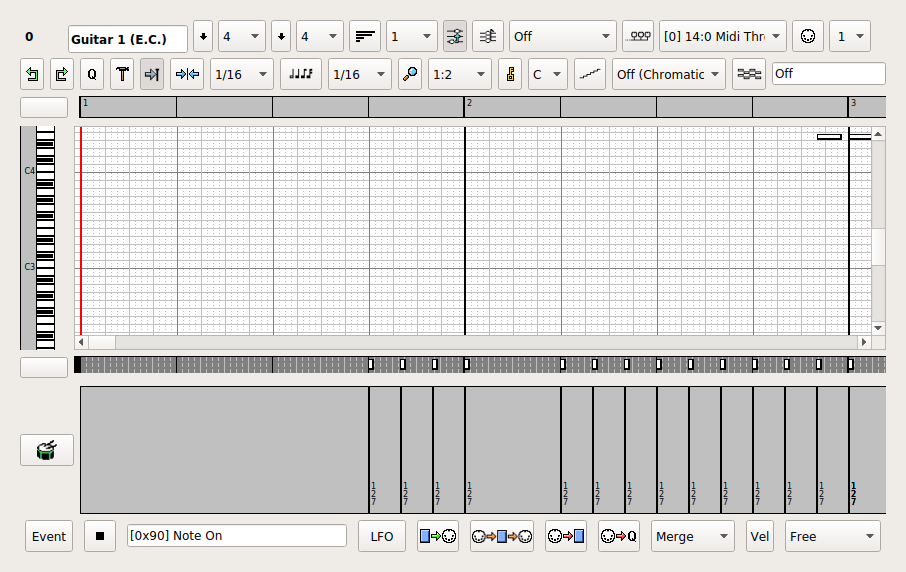
\includegraphics[scale=0.65]{roll.png}
   \caption{MIDI Clock, Manual Option On}
   \label{fig:seq66_midi_clock_4_devices_manual_1}
\end{figure}

   It shows the 16 virtual MIDI output busses that \textsl{Sequencer66} can
   drive.  One needs to use a JACK or ALSA MIDI
   connection application to connect a device on each of those outputs.  The
   fact that the the buss names can
   start with different numbers, depending on the system setup, can complicate
   the playing of MIDI in this manner.  Also, the "user" configuration file can
   change the visible names of the ports, causing further confusion.
   The following elements are present in this dialog:

   \begin{enumber}
      \item \textbf{Index Number}
      \item \textbf{Client Number}
      \item \textbf{Port Number}
      \item \textbf{Buss Name}
      \item \textbf{Port Disabled}
      \item \textbf{Off}
      \item \textbf{On (Pos)}
      \item \textbf{On (Mod)}
      \item \textbf{Clock Start Modulo}
   \end{enumber}

   The format of the left side of the entry listing is like the following:

   \begin{verbatim}
      [4] 4:4 seq66 midi out 4:5
       ^  ^ ^ ^
       |  | | |
       |  | |  -------- Buss name
       |  |  ---------- Port number
       |   ------------ Client number
        --------------- Index number
   \end{verbatim}

   \setcounter{ItemCounter}{0}      % Reset the ItemCounter for this list.

   \itempar{Index Number}{midi clock!index number}
   \index{index number}
   The number in square brackets is an ordinal indicating the position
   of the output buss in the list.
   \index{buss override}
   It can be used with the \texttt{-b --buss --bus} option to redirect all
   output to that one buss, which is useful if only one buss is active, and the
   \textsl{Sequencer66} MIDI song patterns route to non-existent busses.

   \itempar{Client Number}{midi clock!client number}
   \index{client number}
   The number that precedes the colon is the "client number".
   It is useful mainly in ALSA, where clients can have numbers like "14",
   "128", "129", etc.  For native JACK mode, it matches the index number.

   \itempar{Port Number}{midi clock!port number}
   \index{port number}
   The number that follows the colon is the "port number".
   It is useful mainly in ALSA.
   For native JACK mode, it matches the index number.

   \itempar{Buss Name}{midi clock!buss name}
   \index{port name}
   \index{midi clock!port name}
   These labels indicate the output busses (ports) of \textsl{Sequencer66}.
%  They range from \textbf{[1] sequencer66 1} to \textbf{[16] sequencer66 16}
%  in the legacy application, \texttt{sequencer66}.
   They range from \textbf{[1] seq66 1} to \textbf{[16] seq66 16}.
   in native JACK, when manual/virtual ports are active.

   \itempar{Port Disabled}{midi clock!port disabled}
   The \textbf{Port Disabled} clock choice marks a port
   that one does not want to use or that the operating system
   (\textsl{Windows}, I'm looking at \textsl{you}!)
   is locking or disabling that output port.
   Normally, this inaccessible port would cause \textsl{Sequencer66} to exit.
   With the port disabled, the inaccessible port is ignored.

   When the \textsl{Windows} version of \textsl{Sequencer66}
   (\texttt{qpseq66} is first started, it may error out.
   It will then write "erroneous.rc" and "erroneous.usr" configuration
   files, which can be examined to find the offending buss.
%  See \sectionref{fig:qt5_prefs_clock_windows}, it shows this
%  new feature.

   \itempar{Off}{midi clock!off}
   Disables the MIDI \textsl{clock} for the given output buss.
   MIDI output is still sent to those ports, and
   each port that has a device connected to it will play music.
   Some synthesizers may require this setting.
%  For feeding \textsl{Yoshimi} (running in ALSA mode)
%  with MIDI data, we found that this
%  setting is the one that must be made in order for \textsl{Yoshimi} to
%  produce a sound.

   \itempar{On (Pos)}{midi clock!on (pos)}
   MIDI clock will be sent to this buss.
   MIDI Song Position and MIDI Continue will be sent if playback starts
   at greater than tick 0 in Song mode.  Otherwise, MIDI Start will be sent.

   \itempar{On (Mod)}{midi clock!on (mod)}
   MIDI clock will be sent to this buss.
   MIDI Start will be sent, and clocking will begin
   once the Song Position has reached the start modulo of the specified size
   (see the next item's description).
   This setting is used for gear that does not respond to Song Position.

   \itempar{Clock Start Modulo}{midi clock!clock start modulo}
   Clock Start Modulo (1/16 Notes).
   This value starts at 1 and ranges up to 16384, and defaults to 64.
   It is used by the \textbf{On (Mod)} setting discussed above.
   It is the \texttt{[midi-clock-mod-ticks]} option in the \textsl{Sequencer66}
   "rc" file as described in
   \sectionref{subsec:seq66_rc_file_midi_cmt}.

   \itempar{Meta Events}{midi clock!meta events}
   \index{tempo-track-number}
   This section consists of one item, the Tempo Track number.
   It allows the user to move the tempo track from pattern 0 to
   another pattern.  Changing this option is not recommended, since track 1 (0)
   is the official track for tempo events, but \textsl{Sequencer66} allows the
   user to record tempo events to another track.  \textsl{Sequencer66} will
   process tempo events in any pattern.
   \textsl{Not supported yet in the Qt user-interface, but
   it can be set manually in the "rc" configuration file.}

   In addition, the \textbf{Set as Song Tempo Track} button sets this
   track as part of the currently-load MIDI song file, and will be saved when
   exited.  This value will override the global tempo-track value, which is
   stored in the 'rc' configuration file.  However, if 0, it will be ignored,
   so that the global value will take hold.
   See \sectionref{subsec:seq66_rc_file_midi_meta_events}, which discusses this
   setting in the "rc" configuration file.

   One thing to remember about tempo...
   there is a "global" tempo which is saved as part of the song in a SeqSpec
   section.  However, that tempo is not saved in the tempo track.
   In order to do so, one can click the \textbf{Log Tempo} button to write it
   to the tempo track as a tempo event.

\begin{figure}[H]
   \centering 
%  \includegraphics[scale=0.75]{menu/midi-clock-4-devices-manual-0.png}
%  Updated for version 0.93.1:
%  \includegraphics[scale=0.65]{new/midi-clock-4-devices-manual-0.png}
   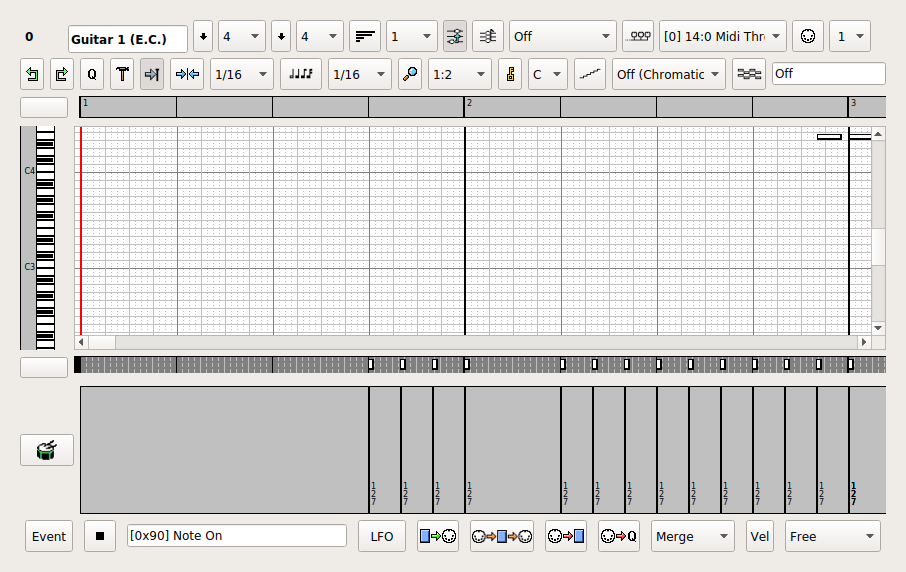
\includegraphics[scale=0.65]{roll.png}
   \caption{MIDI Clock, Manual Option Off (ALSA View, Old Screenshot)}
   \label{fig:seq66_midi_clock_4_devices_manual_0}
\end{figure}

   In the figure above, with "manual-ports" turned off, and
   all of the real (non-virtual) devices that can be driven by MIDI output are
   shown, including the MIDI Thru port, and
%  the MIDI port on the \textsl{E-MU XMidi1x1} USB cable,
   the four ports provided by \textsl{Timidity} on our setup.
%  , and the unlabelled
%  port provided by the \textsl{Yoshimi} synthesizer running in ALSA mode.
%  (However, \texttt{seq66} does show the name "yoshimi" as the client name.)
%  One could theoretically play music through 6 or 7 devices using
%  \textsl{Sequencer66} with this setup.
   (The \textbf{Port Disabled} column is missing from this old screenshot.  We
   need to fix that someday.)

   See \sectionref{subsec:seq66_jack_native_midi},
   for a lot more information about native JACK support, and examples of JACK
   MIDI ports and connections.

   \index{todo!manual alsa gui option}
   There is currently no user-interface item corresponding to the "manual-ports"
   command-line and "rc" configuration file option.
   We should rename this option to "virtual"
   eventually, since it can also apply to JACK MIDI.

\paragraph{Menu / File / Options / MIDI Input}
\label{paragraph:seq66_menu_file_options_midi_input}

   To allow \textsl{Sequencer66} to record MIDI from MIDI devices such as
   controllers and keyboards, the output of the ALSA MIDI recording
   command-line application is relevant:

   \begin{verbatim}
      $ arecordmidi -l
       Port    Client name                      Port name
       14:0    Midi Through                     Midi Through Port-0
       24:0    USB2.0-MIDI                      USB2.0-MIDI MIDI 1
      129:1    seq66                            seq66 midi out 0
      129:2    seq66                            seq66 midi out 1
       . . .   . . .                               . . .
      129:16   seq66                            seq66 midi out 15
   \end{verbatim}

% Should the above be offset re 0, not 1?  Check it out!!!

   We see that we can record MIDI from the MIDI Thru port, from the USB MIDI
   cable, and MIDI from any of the 16 output ports provided by the manual
   port mode of \textsl{Sequencer66}.

   If the "manual-ports" option is turned \textsl{off} (e.g. by using the
   \texttt{-a} option),
   then the only item in the \textbf{MIDI Input} tab is the single MIDI input
   buss provided by \textsl{Sequencer66}:  \textbf{[0] seq66 0}.
   (The figure shown is currently out-of-date.)

% Should the above be offset re 0, not 1?  Check it out!!!

\begin{figure}[H]
   \centering 
%  \includegraphics[scale=0.75]{menu/midi-input-4-devices-manual-1.png}
%  \includegraphics[scale=0.65]{new/midi-input-4-devices-manual-1.png}
   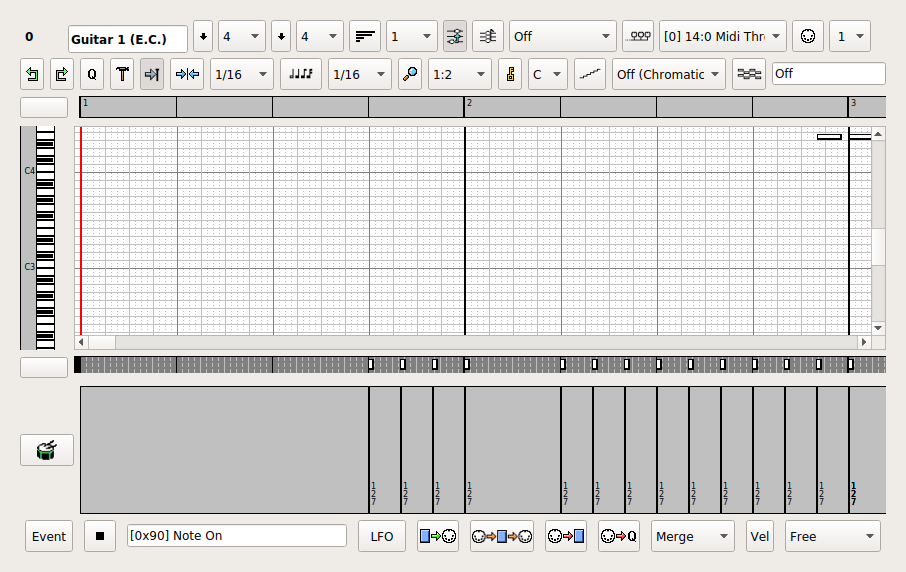
\includegraphics[scale=0.65]{roll.png}
   \caption{MIDI Input, Manual Ports Off (Condensed View)}
   \label{fig:seq66_midi_input_4_devices_manual_1}
\end{figure}

% WE NEED a composite view of the -m, -A, and -a options for ALSA for
% both the Clock and the Input tabs!!!!!

% Check the following out!  I am not 100% certain it is correct!!!
% The above is shown with the -A option.

   Any item checked allows \textsl{Sequencer66} to record MIDI
   from another source,
   which must be connected to this port via
   another application).
%  , or pass it through to the output busses
%  that are configured to allow pass-through
%  (in the Pattern Editor, as discussed in 
%  \sectionref{subsec:seq66_pattern_editor_bottom}.)

   \textbf{Warning:}
   \index{warnings!usr config}
   \index{usr config}
   If the 
   \texttt{[user-midi-bus-definitions]} value in the "user" configuration file
   is non-zero, and the
   corresponding number of
   \texttt{[user-midi-bus-N]} settings are provided, then
   the list of existing hardware will be ignored, and those values will be
   shown instead.
   (This feature can be overridden with the
   \texttt{--reveal-ports} (\texttt{-r}) option.)

%  New in \textsl{Sequencer66} is the option to record MIDI input into
%  more than one pattern based on the MIDI channel, as discussed below.

   If the "auto ALSA ports" option is turned on, via the \texttt{-a} or
   \texttt{--auto-ports} option, then
   the input ports from the system are shown:

\begin{figure}[H]
   \centering 
%  \includegraphics[scale=0.75]{menu/midi-input-4-devices-manual-0.png}
%  \includegraphics[scale=0.65]{new/midi-input-4-devices-manual-0.png}
   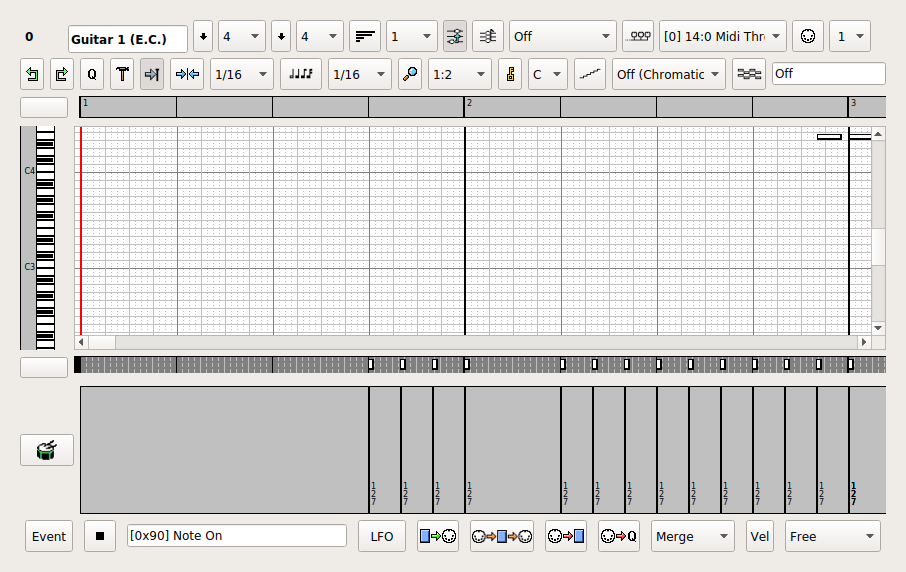
\includegraphics[scale=0.65]{roll.png}
   \caption{MIDI Input, \texttt{-a} Option (Condensed View)}
   \label{fig:seq66_midi_input_4_devices_manual_0}
\end{figure}

   For example, one could check input \#1 to have \textsl{Sequencer66} record
   MIDI from an old-fashioned MIDI keyboard that is connected to another
   USB MIDI cable (the \textsl{E-MU Xmidi}).  If the keyboard didn't have a
   sound generator, one would also want \textsl{Sequencer66} to pass this MIDI
   on to a sound generator, such as a software or hardware synthesizer attached
   to one of the ports shown in
   \figureref{fig:seq66_midi_clock_4_devices_manual_0}.

   \textbf{Warning:}
   \index{warnings!usr config}
   \index{usr config}
   The "user" configuration file can override what is actually
   displayed as hardware.  If you define these sections, they should match your
   hardware exactly, and your hardware should not change from session to
   session.

   Note the two sections of this configuration page:

   \index{input buses}
   \textbf{Input Buses} delineates the MIDI input devices as noted above.
   \index{input options}
   \textbf{Input Options} adds further refinements to MIDI input.

   \index{input by channel}
   \textbf{Record input into sequence according to channel}
   causes MIDI input with multiple channels to be distributed to
   each sequence according to MIDI channel number.
   When disabled, the legacy recording behavior dumps all data into the current
   sequence, regardless of channel.

%  Needs to be clarified!!!

\paragraph{Menu / File / Options / Keyboard }
\label{paragraph:seq66_menu_file_options_keyboard}

   \textsl{Seq24} allows extensive use of
   keyboard shortcuts to make operations go faster than with a mouse,
   and \textsl{Sequencer66} extends that tradition.
   The \textbf{Keyboard} tab (currently in Gtkmm only)
   allows for the configuration of these keyboard shortcuts.

   These settings can also be modified by editing the appropriate "rc"
   configuration file, stored in one of the following directories, depending on
   the operating system:
   
   \begin{verbatim}
         /home/username/.config/sequencer66
         C:/Users/username/AppData/Local/sequencer66
   \end{verbatim}

   \textbf{Warning:}
   \index{keys!gotchas}
   There are a number of "gotchas" to be aware of when assigning keys to the
   fields in the \textbf{Keyboard} tab:

   \begin{itemize}
      \item This configuration dialog is not yet present in the
         \textbf{Qt 5} version of \textsl{Sequencer66}.  For now,
         one has to edit the "rc" file to configure the keystrokes.
         It is easiest to just use the sample \texttt{qpseq66.rc}
         or \texttt{qseq66.rc} from the
         \texttt{data} directory in the source-code package.
         Another option is to just run \textsl{Sequencer66} the first time and
         tweak the "rc" and "usr" files that are created in the directories
         noted above.
         Internally, the Qt key-codes are remapped to Gtk key-codes.
      \item Whenever one of the text fields in this dialog has the focus (and
         that is usually the case), then
         \textsl{any} keystroke, including keys like
         \texttt{Ctrl},
         \texttt{Alt}, and
         \texttt{Super} (also known as Mod4 or the Windows key),
         can alter the value of a
         field to that of the keystroke.  This change is very easy to do
         accidentally!  \textsf{Use the mouse} to move this window and to click
         its \textbf{OK} button!
      \item Some of the keys traditionally used (or used by default) for
         control have been adapted for other uses, and are not configurable.
         One example is \texttt{Ctrl-L}, which brings up the learn mode
         that can be started using the "L" button or the "glearn"
         (group-learn) MIDI control.
         Some other hard-wired keystrokes are the "arrow" keys or "page
         up/down" keys.
      \item \textsl{Sequencer66} has appropriated the
         \index{keys!shift} Shift key so that it
         modifies a click on a pattern so that all of the other patterns are
         \textsl{toggled}.  Therefore, using characters that require the Shift
         key while clicking, such as \texttt{\{} and \texttt{\}}, when used
         to set the \textbf{Replace} function, becomes surprising.
         Instead, look to the remaining keys: \texttt{F11}, \texttt{F12},
         and the "keypad" keys if more options are wanted.  Be sure to
         look at the \textbf{Ext Keys} tab to see what other keys are in use.
         \index{auto-shift}
         Also, for the group-learn feature, the \texttt{Shift} key is 
         automatically enabled, using an "auto-shift" feature.
   \end{itemize}

\begin{figure}[H]
   \centering 
%  \includegraphics[scale=0.65]{new/menu_file_options_keyboard.png}
   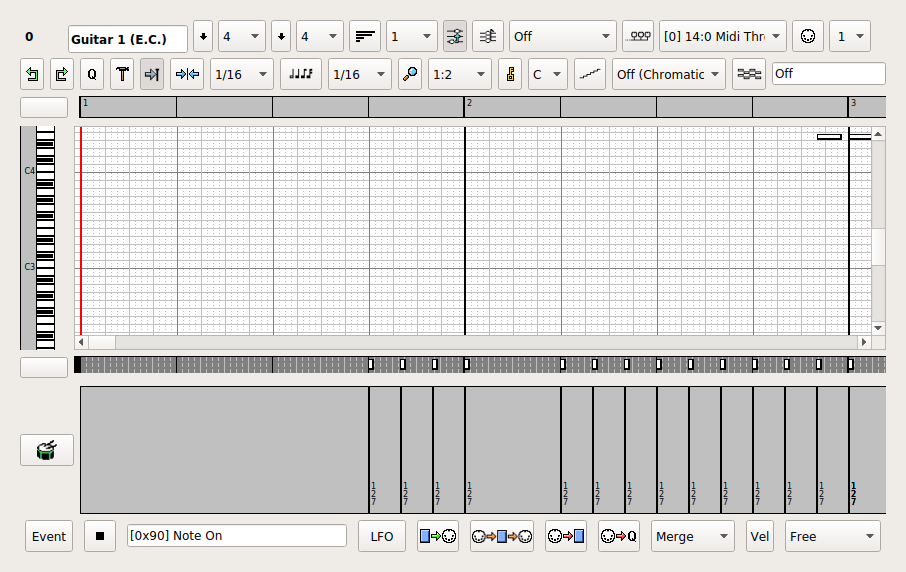
\includegraphics[scale=0.65]{roll.png}
   \caption{File / Options / Keyboard}
   \label{fig:seq66_menu_file_options_keyboard}
\end{figure}

   \texttt{[keyboard-control]}.
   We won't attempt to cover every user-interface item in this busy
   dialog, just the categories.  Some items might be discussed in other parts
   of this manual.

   There are some things to note in the \texttt{[keyboard-control]} section.
   First, it is laid out like the main patterns panel, in an 8 x 4 grid.
   The keys in there correspond directly to the patterns panel slot, and the
   conventional keyboard layout is shown.
   Second, if one is looking for more keys to map to other functions, the
   default layout keeps open the following keys:
   \texttt{9 o l 0 p}.
%  Third, these key-mappings are stored in the
%  \texttt{[keyboard-control]} section of the "rc" configuration file.

   The \texttt{[mute-group]} section is laid out in a similar manner, except
   that the \textbf{upper-case} versions of the keys are used.  Additional keys
   are available for other functions:
   \texttt{( O L ) P}.
   Currently, one must be very carefully about assigning the same key to
   different functions.  Confusion will ensue!  We've done it!
%  Note that these key-mappings are stored in the
%  \texttt{[mute-group]} section of the "rc" configuration file.

%  \index{new!pause}
   \index{pause}
%  If the application has been built with the "pause" option, an
   An additional key definition is shown for the Pause key.
   By default, the Pause key is the period (".").  An old version of
   the "rc" file is automatically fixed to include this new option.
%  (The pause feature can be removed by rebuilding the application
%  after configuring with the \texttt{--disable-pause} option, but
%  why would you want to do that?)

% \begin{figure}[H]
%    \centering 
%    \includegraphics[scale=0.75]{new/keyboard-options-0_9_10_1.png}
%    \caption{File / Options / Keyboard, with Pause}
%    \label{fig:seq66_menu_file_options_keyboard_pause}
% \end{figure}

   \index{pattern edit}
   New features try to achieve being able to edit a pattern using only the
   keyboard.  \textsl{Sequencer66} now supports two modifier keys.
   The first modifier key causes the usual pattern-toggle key (hot-key) for a
   given slot to instead bring up the pattern editor.  By default, this key is
   the equals ("=") key.
   \index{event edit}
   The second modifier key causes the usual
   pattern-toggle key (hot-key) for a given slot to instead bring up the event
   editor.  By default, this key is the minus ("-") key.
   These keys are configurable in the
   \textbf{File / Options / Ext Keys} page.
%  As with the other
%  keys, these keys can be reconfigured to a different set of keys in the
%  \textbf{File / Options / Keyboard} page.

   To continue with a listing of the keyboard options:

   \begin{enumber}
      \item \textbf{Show sequence hot-key labels on sequences}
      \item \textbf{Show sequence numbers on sequences}
      \item \textbf{Control keys [keyboard-group]}
      \item \textbf{Sequence toggle keys [keyboard-control]}
      \item \textbf{Mute-group slots [mute-group]}
      \item \textbf{Learn}
      \item \textbf{Disable}
      \item \textbf{Enable}
   \end{enumber}

   These categories are described below.

   \setcounter{ItemCounter}{0}      % Reset the ItemCounter for this list.

   \itempar{Show key labels on sequence}{keyboard!show labels}
   This option shows the key labels in the lower-right corner of
   each loop/pattern slot in the Patterns window (the main window).
   It is useful for live playback and control of a song.
   It is configurable in the "rc" configuration file.
   It also enables the display of the pattern length, in
   measures, at the top right of the pattern slot.

   \itempar{Show sequence numbers on sequence}{keyboard!sequence numbers}
   \index{new!sequence numbers}
   If this option is on, the
   empty slots in the pattern window show the prospective sequence number.
   See the following figure for one look of this feature.

\begin{figure}[H]
   \centering 
%  \includegraphics[scale=0.75]{pattern-window-with-numbering.png}
%  \includegraphics[scale=0.65]{new/pattern-window-with-numbering.png}
   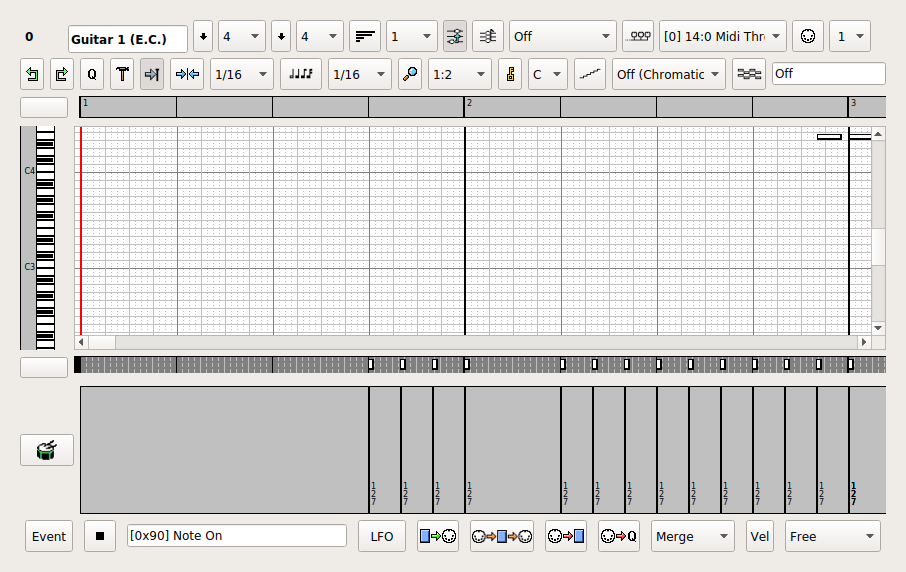
\includegraphics[scale=0.65]{roll.png}
   \caption{Pattern Window with One Kind of Numbering}
   \label{fig:seq66_build_with_numbering}
\end{figure}

   The option also changes the visibility of sequence numbers
   in active sequences and in the Song Editor's names column.
   If one doesn't like it, turn off the option in the "rc" configuration file,
   or try other grid options in the "user" configuration file.

   \itempar{Control keys}{keyboard!control keys}
   \texttt{[keyboard-group]}.
   This block of fields in the \textbf{Options / Keyboard} tab
   provides shortcut keys for many operations of
   \textsl{Sequencer66}.  There is a default mapping built into
   \textsl{Sequencer66}, but open the keyboard options tab to see
   the actual values.
   
%  Some of the old \textsl{Seq24} defaults were ill-advised.

   \begin{enumber}
      \item \textbf{Start}.
      \item \textbf{Stop}.
      \item \textbf{Pause}.
      \item \textbf{Slot Shift}.
      \item \textbf{Snapshot 1}.
      \item \textbf{Snapshot 2}.
      \item \textbf{bpm up}.
      \item \textbf{bpm down}.
      \item \textbf{Replace}.
      \item \textbf{Queue}.
      \item \textbf{Keep queue}.
      \item \textbf{Screenset down}.
      \item \textbf{Screenset up}.
      \item \textbf{Set playing screenset}.
   \end{enumber}

   Some of the keys have positional mnemonic value.  For example,
   for BPM control, the semicolon is at the left (down), and the apostrophe
   is at the right (up).
   Note that the keys definable in this tab are only a subset of the
   various keys that can be used, especially keys used with the
   \texttt{Ctrl} key or other modifier keys.

   \index{slot-shift}
   \index{keys!slot-shift}
   The \textbf{slot shift} key is useful when using pattern grids larger
   than 8 x 4 patterns.  Pressing the slot-shift key basically adds 32 to the
   pattern number of the slot-key that is pressed.
   Not all builds of \textsl{Sequencer66} support this option.

   \index{snapshot}
   \index{keys!snapshot}
   A \textbf{snapshot} is a briefly-preserved state of the patterns.
   One can press a snapshot key, change the state of the patterns for live
   playback, and then release the snapshot key to revert to the state when
   the snapshot key was first pressed.

%  TODO:  Investigate this note from SEQ24:
%
%   Holding 'Alt' will save the state of playing sequences
%   and restore them when 'Alt' is lifted.
%
%   Holding 'Left Ctrl' and 'Alt' at the same time will enable
%   you to flip over to new sequences briefly and then
%   flip right back upon lifting 'Alt'.
%
%	Is this Snapshot 1 versus Snapshot 2?  In Seq24's code, either key
%  does exactly the same thing!


   \index{queue}
   \index{keys!queue}
   To \textbf{queue}
   a pattern means to ready it for playback upon the next repeat
   of a pattern.  A pattern can be armed immediately with a hot-key,
   or it can be queued to play back the next time the pattern repeats.
   A pattern can be queued by holding the queue key (defined in
   \textbf{File / Options / Keyboard / queue}) and pressing a pattern-slot
   hot-key.  Instead of the pattern turning on
   immediately, it turns on at the next repeat of the pattern.

   \index{keep queue}
   \index{keys!keep queue}
   \index{queue!keep}
   \textbf{Keep queue}
   allows the queue to be held without holding
   down the queue button the whole time.  First, press the keep-queue key
   (defined in \textbf{File / Options / Keyboard / Keep queue}).  Now, hitting
   any of the slot hot-keys, no matter how many, sets up the corresponding
   pattern slot to be queued.  Also, in keep-queue mode, clicking on the
   pattern slot will queue the pattern.  The keep-queue mode is disabled by
   hitting the "queue" key again (any currently active queues remain active
   until finished).  There is also a "Q" button to toggle the keep-queue
   status.

   Be sure to note the new option, \textbf{one-shot queue}, in the
   extended-keys section (\sectionref{subsubsec:seq66_patterns_pattern_slot}).

   \itempar{Sequence toggle keys}{keyboard!sequence toggle keys}
   Each of these keys toggles the playing/muting of one of the 32
   loop/pattern boxes.  These keys are layed out logically on the keyboard,
   and can also be shown in each loop/pattern box.  No need to list them all
   here!  Please note that we often call them "shortcut keys" or
   "hot-keys" where the context
   makes it clear that they apply to the armed/unarmed state of a pattern.

   \itempar{Mute-group slots}{keyboard!mute-group slots}
   There can be up to 32 mute-groups.
   \index{playing set}
   When activated, a mute-group
   sets the muted/unmuted status of the current "playing set"
   to the pattern-muting statuses of the selected mute-group.
   Each of these keys operates on the mute-grouping of one of the 32
   stored mute groups.
   These keys are layed out logically on the keyboard.
   No need to list them all here!
   Generally, they are the shifted versions of the
   keyboard keys used as hot-keys for the patterns.
   Note that a mute-group key will be memorized only when
   \textsl{Sequencer66} is in
   \index{group-learn} \textsl{group-learn} mode.

%  \index{mute-group}
%  One thing to explain is just what mute-grouping means.
%  \textsl{Mute groups} are shortcuts to play a defined group of patterns
%  on the current set, while stopping other patterns from the current set, and
%  all patterns from other sets.

   \itempar{Learn}{keyboard!learn}
   \index{group!learn}

   To define the group of patterns for one mute group, press and hold the
   configured Learn key (the \texttt{Insert} key by default,
   the \texttt{Ctrl-L} key, or the "L" button in the user-interface.
   Simultaneously (not needed with the "L" button),
   press one of the mute group keys: \textsl{Sequencer66}
   will save the currently-playing pattern slots into the corresponding mute
   group.
   \index{auto-shift}
   The default mute group keys must be the shifted version of the key,
   but one does not need the \texttt{Shift} key while pressing
   \texttt{Insert} to learn the group, only to trigger it.
   \textsl{Sequencer66} will automatically assign the corresponding key with
   \texttt{Shift} activated.  Try pressing the \texttt{Shift} key in Learn mode
   and see what happens!

%  Now, on some keyboards (like the author's), 
%  the \texttt{Insert} key is a clumsy two-key button.  So, an alternative
%  is to click the \index{L button} \textbf{L button} and release it,
%  then hit the desired mute-group (no need for the \texttt{Shift} key).
%  One can also press \texttt{Ctrl-L} to enter group-learn.

   Group-mute can be globally enabled or disabled (with default keys apostrophe
   \texttt{'} \index{grave} \index{igrave} and igrave or grave \texttt{`}).
   So make sure it is enabled before trying to use it.

%  \itempar{Learn}{keyboard!learn}
%  \index{group!learn}
%  Learn (while pressing a mute-group key).
%  This items sets the key used to initiate a learn mode.
%  It is the \textbf{Insert} key by default.
%  \index{auto-shift}
%  \index{group-learn!auto-shift}
%  When in group-learn mode, the \texttt{Shift} key cannot be hit, so the
%  group-learn mode automatically converts the keys to their shifted versions.
%  \index{shift-lock}
%  \index{group-learn!shift-lock}
%  This feature known as \textsl{shift-lock} or \textsl{auto-shift}.
%  It is new to \textsl{Sequencer66}.
%
%  Also, currently necessary because pressing \texttt{Shift} can clear the
%  arming of the patterns in the current set.

   \itempar{Disable}{keyboard!disable}
   \index{keys!apostrophe}
   It is the \textbf{apostrophe} key by default.
   \index{group!off}
   \index{keyboard!group off}
   This key is the \textsl{group off} key.

   \itempar{Enable}{keyboard!enable}
   \index{keyboard!igrave}
   It is the \textbf{igrave} (back-tick) key by default.
   \index{group!on}
   \index{keyboard!group on}
   This key is the \textsl{group on} key.

\paragraph{Menu / File / Options / Ext Keys }
\label{paragraph:seq66_menu_file_options_ext_keys}

   \texttt{[extended-keys]}.
   A number of additional functions have been added to \textsl{Sequencer66},
   and keystrokes have been provided for those new functions, in the
   \textbf{Ext Keys} page.  This page is needed because the original page is
   completely filled.  The new tab has its own section in the "rc" file.

\begin{figure}[H]
   \centering 
%  \includegraphics[scale=0.75]{menu/menu_file_options_ext_keys_condensed.png}
%  \includegraphics[scale=0.65]{new/menu_file_options_ext_keys_condensed.png}
   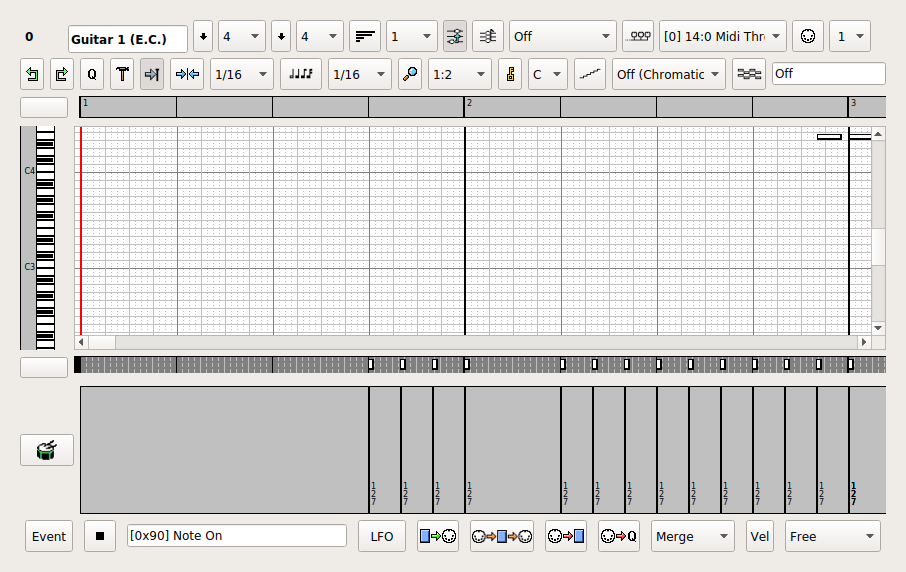
\includegraphics[scale=0.65]{roll.png}
   \caption{File / Options / Ext Keys (Condensed View)}
   \label{fig:seq66_menu_file_options_ext_keys}
\end{figure}

% Currently there is only one block of fields.  New blocks should also be
% marked by "itempar".

   \setcounter{ItemCounter}{0}      % Reset the ItemCounter for this list.

   \itempar{Ext Keys}{keyboard!extended keys}
   This block of fields in the \textbf{Options / Ext Keys} tab
   provides shortcut keys for more operations of \textsl{Sequencer66}, many of
   them ported from \textsl{Seq32} or \textsl{Kepler34}.

   \begin{enumber}
      \item \textbf{Song/Live toggle}.
      \item \textbf{Toggle JACK}.
      \item \textbf{Menu mode}.
      \item \textbf{Follow transport}.
      \item \textbf{Fast forward}.
      \item \textbf{Rewind}.
      \item \textbf{Pointer Position}.
      \item \textbf{Toggle mutes}.
      \item \textbf{Tap BPM}.
      \item \textbf{Song Record}.
      \item \textbf{One-shot Queue}.
         This new feature allows one-shot queuing of a pattern.
   \end{enumber}

   Most of these extended keys implement operations performed with button
   presses.  Some of the new keystrokes may not have a corresponding
   button.
   These values are saved as the \texttt{[extended-keys]} section of the "rc"
   configuration file.
%  However, not all builds of \textsl{Sequencer66} will
%  support the new keys.  Some of the new features can be enabled or disabled
%  during the build-configure step, and one's favorite Linux distro may decide to
%  disable some features.
%  An option might be disabled during the build process.
%  In this case, although the values will still be
%  stored in the "rc" file, they will be disabled or missing in this tab:

\begin{figure}[H]
   \centering 
%  \includegraphics[scale=0.65]{menu/menu_file_options_ext_keys_disabled.png}
   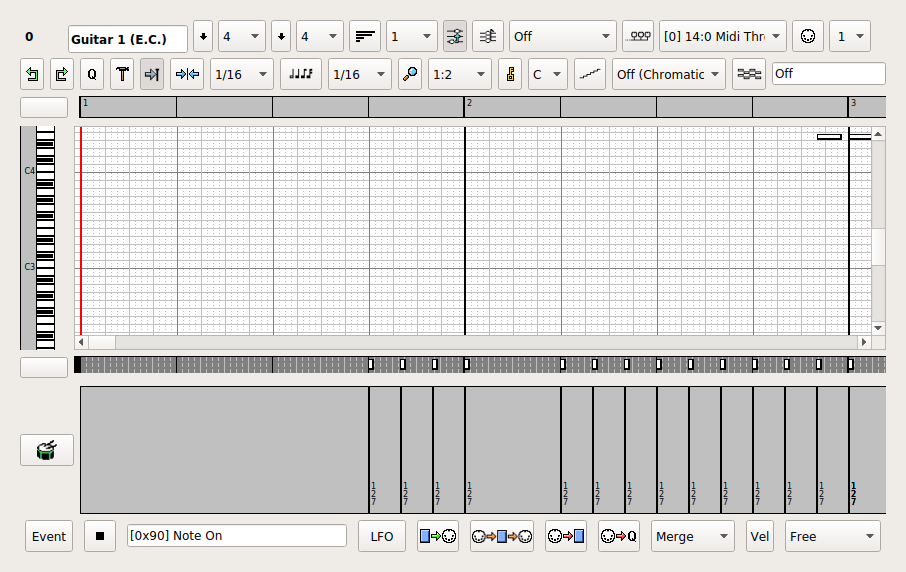
\includegraphics[scale=0.65]{roll.png}
   \caption{File / Options / Ext Keys (Disabled)}
   \label{fig:seq66_menu_file_options_ext_keys_disabled}
\end{figure}

   \index{song mode}
   Note the \textbf{Song/Live toggle} key.
   The \textsl{song mode} normally is in effect only when playback is started
   from the \textbf{Song Editor}.  Now this mode can be used from any
   window, if enabled by pressing this key.  There is also
   a button in the main window for this function, which shows the current state
   of this flag.  Note that this flag is also stored in the "rc" configuration
   file, as well as this hot-key value, which defaults to \texttt{F1}.

   \index{toggle JACK}
   \index{JACK toggle}
   The \textsl{JACK mode} is set via the
   \textbf{File / Options / JACK / JACK Connect} or 
   \textbf{JACK Disconnect} buttons.
%  But, if \textsl{Sequencer66} is built for
%  using the \textsl{Seq32} JACK support, then
   This keystroke will toggle between JACK connect and JACK disconnect.
%  Note that, with this kind of build,
   The \textbf{Song Editor} will also have a \textbf{JACK} button.
   The hot-key for this function defaults to \texttt{F2}.

   \index{menu mode}
   The \textsl{menu mode} indicates if the main menu of the
   main window is accessible or not.  It is disabled during playback
   so that more hot-keys can be used without triggering menu functions.
   It can also be disabled by the user; the default hot-key is \texttt{F3}.
   This feature is needed because the original \textsl{Seq24} had numerous
   conflicts between the menu key bindings and the default key bindings for the
   main window.

%  Here is Stazed's explanation of the feature, mildly edited:
%
%  \begin{quotation}
%     \textsl{"why disabling is needed when playing"}
%     The original seq24 had numerous conflicts between the menu key binding
%     and the default seq24 key binding for the mainwind sequence triggers.
%     For example: Ctrl-q (quits the program without prompt). If you place a
%     sequence in the default 'q' slot, you cannot use it with Ctrl-l or Ctrl-r
%     (default replace or queue) because the menu grabs the keys. Same goes for
%     the Alt-l or Alt-r (default snapshot 1 or 2). Try same as above with
%     Alt-f, Alt-v, Alt-h, Ctrl-n, Ctrl-o...  etc. So I just shut off all the
%     menus by default when playing because it seems that they should not be
%     needed then... especially in a live performance.
%
%     \textsl{"why a button?"}
%     On occasion I wanted to use the mainwnd key binding when stopped to set
%     the sequences to be ready before starting. It's also a sort of safety
%     feature as well, just toggle the menus off before going live so that you
%     don't hit Ctrl-q, Ctrl-n etc. forgetting things are not playing....
%  \end{quotation}

   \index{follow transport}
   \textsl{Follow transport} is a feature ported from \textsl{Seq32}.
   The default key is \texttt{F4}.
   It determines if \textsl{Sequencer66} follows JACK transport.

   \index{fast forward}
   \textsl{Fast forward} is a feature ported from \textsl{Seq32}.
   The default key is \texttt{F5}.
   While this key is held, the song pointer will fast-forward
   through the song.
   This feature does not have a corresponding button.
   This feature requires that the \textsl{Seq32} transport option be
   enabled at build time.

   \index{rewind}
   \textsl{Rewind} is a feature ported from \textsl{Seq32}.
   The default key is \texttt{F6}.
   While this key is held, the song pointer will rewind.
   This feature does not have a corresponding button.
   This feature requires that the \textsl{Seq32} transport option be
   enabled at build time (and now that is the default).
   Be sure not to use the following keys, which are already
   hardwired for other functions in the Pattern Editor and Song Editor:

   \begin{itemize}
      \item \texttt{p}.  Paint mode.
      \item \texttt{x}.  Escape paint mode.
   \end{itemize}

   \index{pointer position}
   \textsl{Pointer position} is a feature ported from \textsl{Seq32}.
   The default key is \texttt{F7}.
   When this key is pressed, the song pointer will move to the
   current position of the mouse, snapped.
   This feature does not have a corresponding button.

   \index{toggle mutes}
   \textsl{Toggle mutes} toggles the mute status of every
   pattern on every screen-set.  It corresponds to the
   \textbf{Edit / Toggle mute all tracks} or the 
   \textbf{Song / Toggle All Tracks}
   menu entries.  There is also a button in the main window for this function,
   which shows the current state of this flag.  Note that this
   hot-key value is stored in the "rc" configuration file, and
   defaults to \texttt{F8}.

   \index{tap bpm}
   \textsl{Tap bpm} allows the user to "tap" in time with some
   other music, and see the tap sequence translated into beats/minute (BPM).
   There is also a "0" button for this function.
   After 5 seconds, this feature resets automatically, so the user can try
   again if not satisfied.  At least two taps are needed for the
   BPM to be registered.

% VERIFY and the UNCOMMENT
%
%  Tap BPM causes events to be logged to the tempo track which is the first
%  track (track 0) by default.

\paragraph{Menu / File / Options / Mouse }
\label{paragraph:seq66_menu_file_options_mouse}

   This item selects the mouse-interaction method.

\begin{figure}[H]
   \centering 
%  \includegraphics[scale=0.65]{menu/menu_file_options_mouse_condensed.png}
   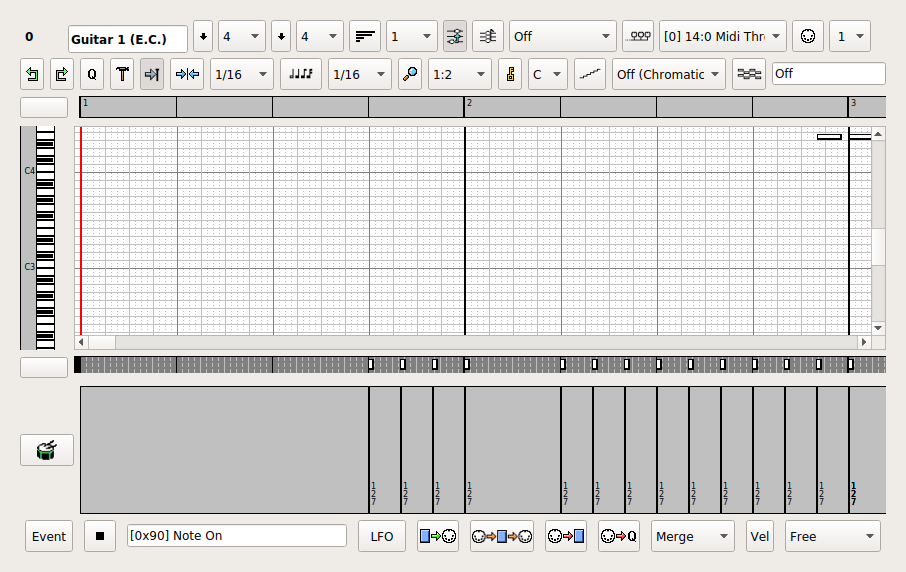
\includegraphics[scale=0.65]{roll.png}
   \caption{File / Options / Mouse (Condensed View)}
   \label{fig:seq66_menu_file_options_mouse}
\end{figure}

   \index{interaction method}
   \index{mouse interaction}
   \textbf{Interaction Method}

   The default mouse interaction method is \textbf{Seq24 (original style)}.
   The alternate mouse interaction method is \textbf{Fruity (similar to a
   certain well known sequencer)}.
   The "Fruity" interaction method
   is currently only available in the Gtkmm-2.4 user-interface, and it
   is not comprehensive.
   For Qt 5, only the original style is available, at this time.

   \index{mouse!fruity}
   The alternate method is presumably that of the \textsl{Fruity Loops}
   (now \textsl{FL Studio}) sequencer.  The fruity mode seems to involve the
   following rules:

   \begin{itemize}
      \item \textbf{Left-click left side}.
         Begin a grow/shrink operation for the left side.
         However, even in \textsl{Seq24}, this action is \textsl{broken}.
         It does allow one to move the note, however.
      \item \textbf{Left-click right side}.
         Begin a grow/shrink operation for the right side.
      \item \textbf{Left-click middle}.
         Move the object.  To clarify, each note image
         has an invisible "handle" on the left or the right side, with the
         middle providing a third area of interaction in the "fruity" mode.
      \item \textbf{Left-click}.
         Add an event if nothing selected.
      \item \textbf{Middle-click}.
         Split the note?
   \end{itemize}

   There may be a few more rules to add, when time allows.

% This paragraph needs to be moved to the pattern editor.

   The \textsl{Seq24} note-editing style is as expected for basic
   actions such as selecting and moving notes using the left mouse button.
   Drawing a note or event is a bit different, in that one must first
   \textsl{click and hold} the right mouse button, and then
   \textsl{click and drag} the right mouse button to insert notes,
   Notes are inserted to be at the current length and grid-snap values for
   the sequence editor for as long as the buttons are pressed.
   Notes are inserted only up to the specified sequence length.
   Once notes are inserted, moving the mouse with the left button still
   held down moves the notes to the new note value of the mouse.
   If one releases the left button, then presses and holds it again,
   more notes will be added in the same way.
   This is unconventional, but a powerful way to layer notes in a short
   sequence.
   We call it the
   \index{draw mode}
   \index{mode!draw}
   "draw mode" or
   \index{paint mode}
   \index{mode!paint}
   "paint mode".
   Drawing/painting can also be done while the sequence is playing,
   and notes will be added to be played the next time the progress bar crosses
   them.

%  \index{sequencer66 options}
%  The \textbf{Sequencer66 Options} section contains a couple of new options.

   \index{keys!Mod4}
   \index{mouse!Mod4}
   \label{new_mod4_mode}
   \textbf{Mod4 key preserves add (paint) mode in song and pattern editors}.
   In order to work with trackpads that don't permit simultaneous left
   and right clicks, the
   "Seq24" mode of mouse interaction can be modified in the
   Pattern or Song editors so that the Mod4 key (Super or Windows key)
   can be pressed when releasing the right mouse button.
   This keeps the mouse in note-add mode.
   Another right-click, without pressing Mod4, will exit this mode.

%  The reason for this feature is the crummy FocalTech touchpad on one of
%  the author's laptops.  This trackpad seems to have only a single button,
%  which the driver interprets as left or right depending where the finger
%  is when it is clicked.  There's no way to click the right and left
%  buttons at the same time.  There's no way to make a middle-click action.
%  What a crock!

   This option will not interfere with the Mod4 key being set
   in the \textbf{Keyboard} option tab, since the keys there mainly apply to
   the Patterns Panel (main window), not the pattern-editor window.

   \index{mouse!split mode}
   \label{new_split_mode}
   Middle click splits song triggers at nearest snap (instead of
   the halfway point).
% Move this section to the right place and simply create a section-reference to
% it here.

   \index{paint mode}
   Another way to turn on the paint mode has been added.
%  , based on a feature
%  found in a patch that someone posted about in some mailing list somewhere on
%  the internet.
   To turn on the paint mode, press the
   \index{keys!p}
   \texttt{p} key while in the sequence editor.
   This is just like pressing the right mouse button, but the draw/paint mode
   stays on.
   To get out of the paint mode, press the
   \index{keys!x}
   \texttt{x} key while in the sequence editor.
   These keys, however, do not work while the sequence is playing.

%  \index{todo:extend mouse support}
%  These convenience options are limited to the
%  pattern/sequence editor window and the performance editor window, and may
%  need some heavier testing.
   Note that some \textsl{Sequencer66} windows
   can use the ctrl-left-click as a middle click. 
 
\paragraph{Menu / File / Options / Jack Sync}
\label{paragraph:seq66_menu_file_options_jack_sync}

   This tab sets up JACK transport, if \textsl{Sequencer66}
   was built with JACK support.
%  It now also supports native JACK MIDI.
   This tab also sets up options for using LASH session management, \textsl{if}
   \textsl{Sequencer66} was built with LASH support, which is no longer the
   default, even though it is shown in the figure below.

\begin{figure}[H]
   \centering 
%  \includegraphics[scale=0.75]{menu/menu_file_options_jack_sync.png}
%  \includegraphics[scale=0.75]{new/menu_file_options_jack_sync.png}
%  \includegraphics[scale=0.65]{jack/menu_file_options_jack_sync.png}
   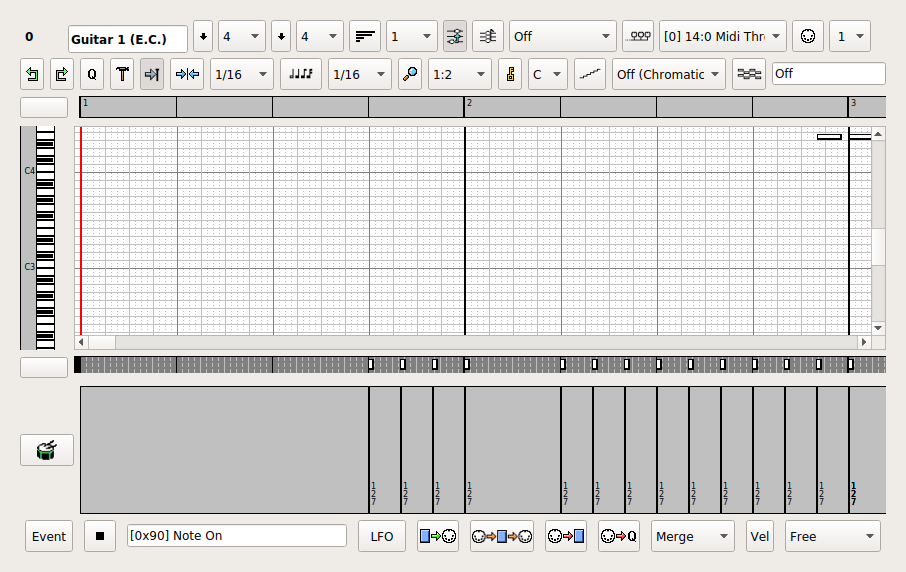
\includegraphics[scale=0.65]{roll.png}
   \caption{File / Options / JACK}
   \label{fig:seq66_menu_file_options_jack_sync}
\end{figure}

   The main sections in this dialog are:

   \begin{enumber}
      \item \textbf{JACK Transport/MIDI}
      \item \textbf{JACK Start Mode}
      \item \textbf{JACK Transport Connect and Disconnect}
      \item \textbf{LASH Options}
   \end{enumber}

   \setcounter{ItemCounter}{0}      % Reset the ItemCounter for this list.

   \itempar{Transport/MIDI}{jack sync!transport/midi}
   These settings are stored in the "rc" file settings group
   \texttt{[jack-transport]}.
   See \sectionref{subsec:seq66_rc_file_jack_transport},
   which describes this configuration option.
   This items collects the following settings:

   \begin{itemize}
      \item \textbf{Jack Transport}.
         \index{JACK!transport}
         Enables slave synchronization with JACK Transport.
         The command-line option is \texttt{--jack-transport}.
         The behavior of this mode of operation is perhaps not quite
         correct.  Even as a slave, \textsl{Sequencer66} can start and
         stop playback.
         Note that this option cannot be disabled via the mouse if the
         \textbf{Transport Master} option is enabled.  Disable that one first.
      \item \textbf{Transport Master}.
         \index{JACK!transport master}
         \textsl{Sequencer66} will attempt to serve as the JACK Master.
         The command-line option is \texttt{--jack-master}.
         \textbf{Tip}:
         \textsl{Sequencer66} generally works better as JACK Master.
         If this option is enabled the \textbf{JACK Transport} option is
         automatically enabled as well.
      \item \textbf{Master Conditional}.
         \index{JACK!master conditional}
         \textsl{Sequencer66} will fail to serve as the JACK Master if there is
         already a Master.
         The command-line option is \texttt{--jack-master-cond}.
         If this option is enabled the \textbf{JACK Transport} option is
         automatically enabled as well.
      \item \textbf{Native JACK MIDI}.
         \index{JACK!native midi}
         This option is for the \texttt{seq66} version of
         \textsl{Sequencer66}.
         If set, MIDI input and output use native JACK MIDI,
         rather than ALSA.  However, if JACK is not running on the
         system, then \texttt{seq66} will fall back to ALSA mode.
         The command-line option is \texttt{--jack-midi}.
   \end{itemize}

%  Note that there are long-standing issues with the JACK support of
%  \textsl{Seq24}, and \textsl{Sequencer66} currently inherits some of them,
%  in spite of some bug fixes.  Generally, if one experiences issues in
%  transport control, try making one of the other sequencer applications the
%  JACK Master.
%  If one starts \textsl{Sequencer66} in JACK mode without JACK running,
%  it will take a little while for \textsl{Sequencer66} to start up, and it
%  will fall back to ALSA usage.

   If one makes a change in the JACK transport settings, it is best to
   then press the \textbf{JACK Transport Disconnect} button, then the
   \textbf{JACK Transport Connect} button.  Another option is to restart
   \textsl{Sequencer66}... the settings are automatically saved when
   \textsl{Sequencer66} exits.

   \itempar{JACK Start mode}{jack sync!start mode}
   This item collects the following settings, also stored in the "rc" file
   settings group \texttt{[jack-transport]}.

   \begin{itemize}
      \item \textbf{Live Mode}.
         \index{JACK!live mode}
         \index{live mode}
         \index{non-playback mode}
         Playback will be in live mode.  Use this option to allow muting and
         unmuting of patterns.  This option might also be called "non-song
         mode".
         The command-line option is \texttt{--jack-start-mode 0}.
      \item \textbf{Song Mode}.
         \index{JACK!song mode}
         \index{song mode}
         \index{playback mode}
         \index{performance mode}
         Playback will use only the Song Editor's data.
         The command-line option is \texttt{--jack-start-mode 1}.
   \end{itemize}

   \textsl{Sequencer66} also selects the playback modes
   according to which window started the playback,
   reverting back to legacy \textsl{Seq24} behavior.
   \textsl{The main window}, or pattern
   window, causes playback to be in live mode.  The user can arm and mute
   patterns in the main window by clicking on sequences, using their hot-keys,
   and by using the group-mode and learn-mode features.
   The song editor causes playback to be in performance mode, also known as
   "playback mode", or \textbf{Song} mode.

   \itempar{Connect}{jack sync!connect}
   Connect to JACK Sync.
   This button is useful to restart JACK sync when making changes to it,
   or when \textsl{Sequencer66} was started in ALSA mode.

   \itempar{Disconnect}{jack sync!disconnect}
   Disconnect from JACK Sync.
   This button is useful to stop JACK sync when making changes to it.

   \itempar{LASH Options}{lash!option}
   Currently contains only one item, which enables the usage of LASH session
   management.  Currently, \textsl{Sequencer66} needs to be restarted to
   complete the enabling or disabling of LASH support.  Like the rest of the
   options, this one is written to the "rc" configuration file.
   However, LASH is no longer supported in the default build.

   Finally, there is a new button (labelled \textsl{Master} in the following
   figure) in the main window to bring up directly the
   \textbf{JACK} (or \textbf{JACK/LASH}) page.

\begin{figure}[H]
   \centering 
%  \includegraphics[scale=0.75]{menu/menu_file_options_jack_sync.png}
%  \includegraphics[scale=0.65]{new/main_master_button.png}
   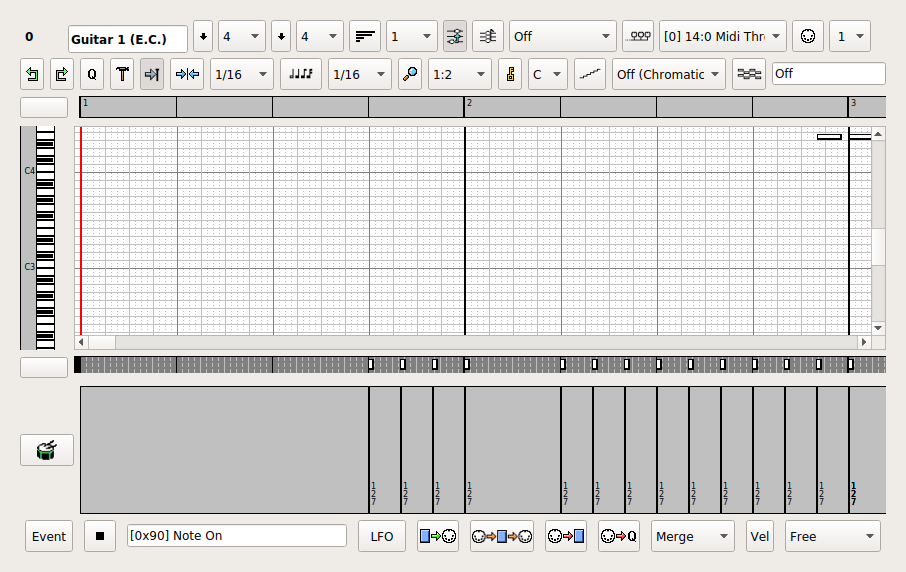
\includegraphics[scale=0.65]{roll.png}
   \caption{JACK Connection Button}
   \label{fig:seq66_main_master_button}
\end{figure}

   This button not only brings up the JACK page, but also shows the current
   status of the MIDI connection:
   \textbf{Master} (JACK Transport Master),
   \textbf{Slave} (JACK Transport Slave),
   \textbf{JACK} (native JACK MIDI, overrides any transport label),
   and \textbf{ALSA} (overridden by any transport label).
   \index{jack page!ctrl-p}
   \index{keys!ctrl-p}
   The \texttt{Ctrl-P} key will also bring up this page.

   One thing to note is that, while playing, the JACK/ALSA button is disabled.
   However, one can still get to the JACK options via the main File menu.
   JACK connection and disconnection are disabled during playback, but the
   buttons don't yet reflect that status.

\subsection{Menu / Edit}
\label{subsec:seq66_menu_edit}

   The \textbf{Edit} menu has undergone some expansion lately.

\begin{figure}[H]
   \centering 
%  \includegraphics[scale=0.65]{new/menu_edit_0_90.png}
   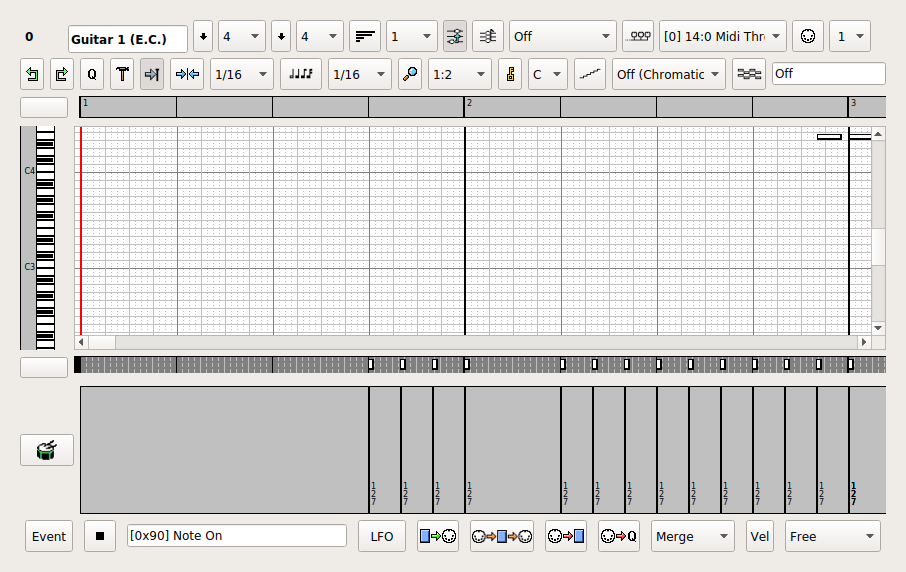
\includegraphics[scale=0.65]{roll.png}
   \caption{Edit Menu}
   \label{fig:seq66_menu_edit_0_90}
\end{figure}

   \begin{enumber}
      \item \textbf{Preferences...} (only in the Qt user-interface)
      \item \textbf{Song Editor...}
      \item \textbf{Apply song transpose}
      \item \textbf{Clear mute groups}
      \item \textbf{Reload mute groups}
      \item \textbf{Mute all tracks}
      \item \textbf{Unute all tracks}
      \item \textbf{Toggle mute all tracks}
   \end{enumber}

   \setcounter{ItemCounter}{0}      % Reset the ItemCounter for this list.

   \itempar{Preferences}{edit!preferences}
   In the Qt user-interface, there is a \textbf{Preferences} menu entry,
   corresponding to the Gtkmm user-interface's \textbf{File / Options}
   menu entry.

   \itempar{Song Editor}{edit!song editor}
   \index{song editor}
   This item is the same as the 
   \textbf{View / Song Editor toggle} menu entry.  It toggles the presence of
   the main song editor.

   \itempar{Apply song transpose}{edit!song transpose}
   \index{song transpose}
   Selecting this item applies the song transposition value to
   \textbf{all} sequences/patterns that are marked as transposable.
   (Normally, drum tracks are \textsl{not} transposable).
   This actively changes the note/pitch value of all note and aftertouch events
   in the pattern.
%  Once the transpositions are done, the transposition value is set to 0.
   For the setting of song transpose, see
   \sectionref{sec:seq66_song_editor}, for more information.
   Also note that transpose can be enabled in the patterns panel for each
   pattern (see \sectionref{subsubsec:seq66_patterns_pattern_filled}) and
   in the sequence editor
   (see \sectionref{sec:seq66_pattern_editor}).

   \itempar{Clear mute groups}{edit!clear mute groups}
   \index{mute groups}
   A feature of \textsl{Seq24} and \textsl{Sequencer66} is that the mute groups
   are saved in both the "rc" file
   (see \sectionref{subsec:seq66_rc_file_mute_group})
   \textsl{and} in the "MIDI" file
   (see \sectionref{subsec:legacy_midi_format}).

   This menu entry clears them. If this resulted in any mute-group sequences
   status being set to false, then the user is prompted to save the MIDI
   file, so that it will no longer have any
   mute-group information.  And then, if the
   application exits, the cleared mute-group information is also saved to
   the "rc" file.
%  We'd like to be able to handle the "rc" and "MIDI"
%  mute-groups separately in the future.

   \itempar{Reload mute groups}{edit!load mute groups}
   \index{rc!mute groups}
   This menu entry reloads the mute-groups from the "rc" file.
   So, if one loads a MIDI file that has its own mute groups that one does not
   like, this command will restore one's favorite mute-grouping from the "rc"
   file.

   \itempar{Mute all tracks}{edit!mute all tracks}
   \index{mute all}
   This menu entry, available only in \textbf{Live} mode,
   immediately mutes \textsl{all} patterns in the entire song.

   \itempar{Unmute all tracks}{edit!unmute all tracks}
   \index{unmute all}
   This menu entry, available only in \textbf{Live} mode,
   immediately unmutes \textsl{all} patterns in the entire song.

   \itempar{Toggle mute all tracks}{edit!toggle all tracks}
   \index{toggle mute all}
   This option toggles the mute/armed status of \textbf{all} tracks.
   It is only available in \textbf{Live} mode, which overrides \textbf{Song}
   mode even if the Song Editor is focussed.
   \textsl{Do not confuse it with the main \textbf{Mute} button, which toggles the
   status only of the tracks that are armed and remembers them.}

\subsection{Menu / View}
\label{subsec:seq66_menu_view}

   If the "allow two perfedits" option is turned off in the "user"
   configuration file, this menu item has only one entry, \textbf{Song Editor}, 
   which is already covered by a button at the bottom of the Patterns
   window.  Selecting this item bring up the Song Editor window.
   See \figureref{fig:song_editor_window}.
   The Song Editor window can also be brought up via the
   \index{song editor!ctrl-e}
   \index{keys!ctrl-e}
   Ctrl-E key.

   If the \textbf{allow two perfedits} option is turned on in the "user"
   configuration file, this menu item has two entries,
   as shown in the following figure:

\begin{figure}[H]
   \centering 
%  \includegraphics[scale=0.65]{menu/menu_view-dual-song-editors.png}
   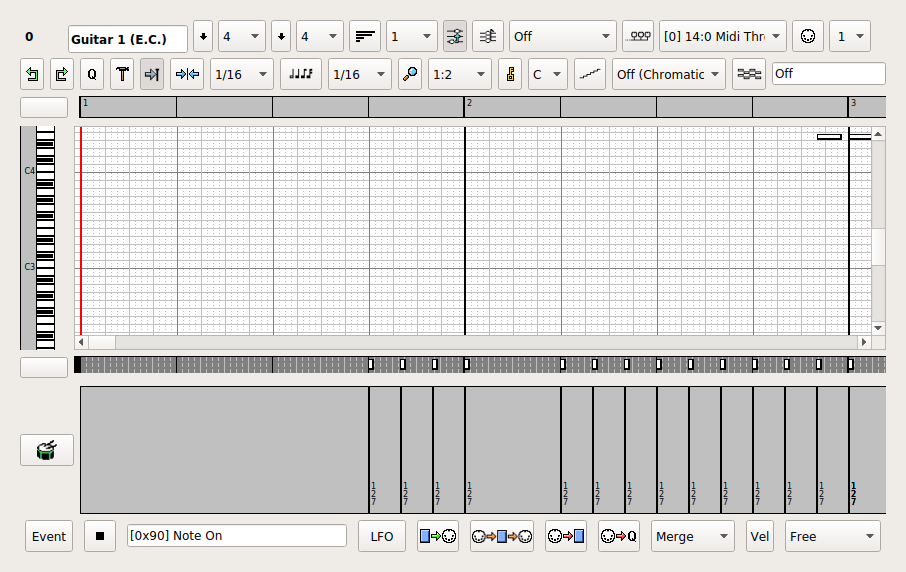
\includegraphics[scale=0.65]{roll.png}
   \caption{Dual Song Editor Entries in View Menu}
   \label{fig:seq66_menu_view_song_editors}
\end{figure}

   Note that only the first Song Editor has a user-interface button and
   a hot-key.  Also note that there can be issues bringing up the second
   song-editor with the hot-key.  The menu entry will always work.
   If two song editors are up, they each track any changes made in the other
   song editor.  But the main purpose of two song editors is to arrange two
   different parts of the performance at the same time when not all the
   patterns will fit in one window.

   In the Qt user-interface, there is a \textbf{Song} tab in the main window.
   But there is also song-editor button in the main window
   and a menu entry in \textbf{Edit / Song Editor},
   which bring up a separate window for the song-editor.
   Do not try to use both windows for song-editing at the same time; they
   are not synchronized.

\subsection{Menu / Help / About...}
\label{subsec:seq66_menu_about}

   This menu entry shows the "About" dialog.

\begin{figure}[H]
   \centering 
%  \includegraphics[scale=0.75]{menu/menu_help_about.png}
%  \includegraphics[scale=0.65]{new/menu_help_about.png}
   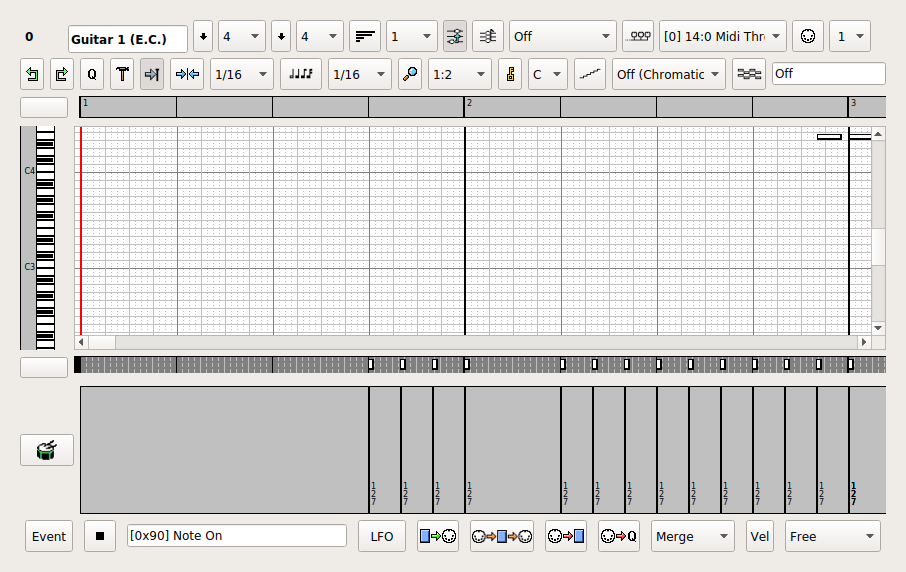
\includegraphics[scale=0.65]{roll.png}
   \caption{Help / About}
   \label{fig:seq66_menu_help_about}
\end{figure}

   The Qt version is slightly different.
%  That dialog provides access to the credits for the program, including the
%  authors and the project documentors.  It has recently been updated
%  to show Git version-control information as well.

\begin{figure}[H]
   \centering 
%  \includegraphics[scale=0.65]{menu/menu_help_credits.png}
   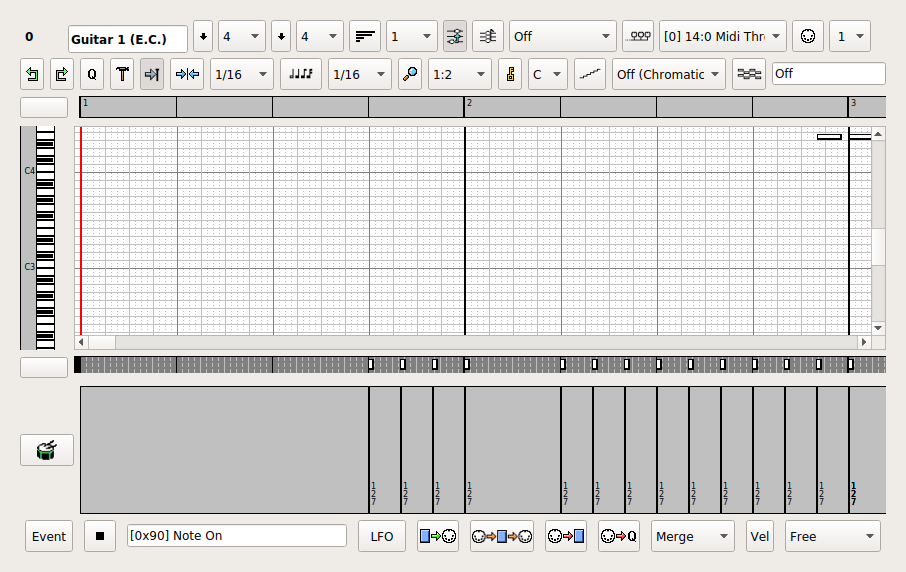
\includegraphics[scale=0.65]{roll.png}
   \caption{Help Credits}
   \label{fig:seq66_menu_help_credits}
\end{figure}

   Shows who has worked on the program, with the original author at the top
   of the list.

\begin{figure}[H]
   \centering 
%  \includegraphics[scale=0.65]{menu/menu_help_doc.png}
   \includegraphics[scale=0.65]{roll.png}
   \caption{Help Documentation}
   \label{fig:seq66_menu_help_doc}
\end{figure}

   Shows who has documented this project.

\subsection{Menu / Help / Build Info...}
\label{subsec:seq66_menu_build_info}

   This menu entry shows the "Build Info" dialog.  This list of
   build options enabled in the current application is the same list
   that it generated via this command line:

   \begin{verbatim}
      $ seq66 --version
   \end{verbatim}

\begin{figure}[H]
   \centering 
%  \includegraphics[scale=0.50]{new/menu_help_build_info.png}
   \includegraphics[scale=0.65]{roll.png}
   \caption{Help / Build Info}
   \label{fig:seq66_menu_help_build_info}
\end{figure}

%-------------------------------------------------------------------------------
% vim: ts=3 sw=3 et ft=tex
%-------------------------------------------------------------------------------
